\documentclass[14pt,a4paper,report]{report}
\usepackage[a4paper, mag=1000, left=2.5cm, right=1cm, top=2cm, bottom=2cm, headsep=0.7cm, footskip=1cm]{geometry}
\usepackage[utf8]{inputenc}
\usepackage[english,russian]{babel}
\usepackage{indentfirst}
\usepackage[dvipsnames]{xcolor}
\usepackage[colorlinks]{hyperref}
\usepackage{listings} 
\usepackage{fancyhdr}
\usepackage{caption}
\usepackage{amsmath}
\usepackage{latexsym}
\usepackage{graphicx}
\usepackage{amsmath}
\hypersetup{
	colorlinks = true,
	linkcolor  = black
}

\usepackage{titlesec}
\titleformat{\chapter}
{\Large\bfseries} % format
{}                % label
{0pt}             % sep
{\huge}           % before-code


\DeclareCaptionFont{white}{\color{white}} 

% Listing description
\usepackage{listings} 
\DeclareCaptionFormat{listing}{\colorbox{gray}{\parbox{\textwidth}{#1#2#3}}}
\captionsetup[lstlisting]{format=listing,labelfont=white,textfont=white}
\lstset{ 
	% Listing settings
	inputencoding = utf8,			
	extendedchars = \true, 
	keepspaces = true, 			  	 % Поддержка кириллицы и пробелов в комментариях
	language = Python,            	 	 % Язык программирования (для подсветки)
	basicstyle = \small\sffamily, 	 % Размер и начертание шрифта для подсветки кода
	numbers = left,               	 % Где поставить нумерацию строк (слева\справа)
	numberstyle = \tiny,          	 % Размер шрифта для номеров строк
	stepnumber = 1,               	 % Размер шага между двумя номерами строк
	numbersep = 5pt,              	 % Как далеко отстоят номера строк от подсвечиваемого кода
	backgroundcolor = \color{white}, % Цвет фона подсветки - используем \usepackage{color}
	showspaces = false,           	 % Показывать или нет пробелы специальными отступами
	showstringspaces = false,    	 % Показывать или нет пробелы в строках
	showtabs = false,           	 % Показывать или нет табуляцию в строках
	frame = single,              	 % Рисовать рамку вокруг кода
	tabsize = 2,                  	 % Размер табуляции по умолчанию равен 2 пробелам
	captionpos = t,             	 % Позиция заголовка вверху [t] или внизу [b] 
	breaklines = true,           	 % Автоматически переносить строки (да\нет)
	breakatwhitespace = false,   	 % Переносить строки только если есть пробел
	escapeinside = {\%*}{*)}      	 % Если нужно добавить комментарии в коде
}

\begin{document}

\def\contentsname{Содержание}

% Titlepage
\begin{titlepage}
	\begin{center}
		\textsc{Санкт-Петербургский Политехнический 
			Университет Петра Великого\\[5mm]
			Кафедра компьютерных систем и программных технологий}
		
		\vfill
		
		\textbf{Отчёт по лабораторной работе №1\\[3mm]
			Курс: «Базы данных»\\[3mm]
			Тема: «Знакомство с ORM на примере Django»\\[35mm]
			}
	\end{center}
	
	\hfill
	\begin{minipage}{.5\textwidth}
		Выполнил студент:\\[2mm] 
		Бояркин Никита Сергеевич\\
		Группа: 43501/3\\[5mm]
		
		Проверил:\\[2mm] 
		Мяснов Александр Владимирович
	\end{minipage}
	\vfill
	\begin{center}
		Санкт-Петербург\\ \the\year\ г.
	\end{center}
\end{titlepage}

% Contents
\tableofcontents
\clearpage

\chapter{Лабораторная работа №1}

\section{Цель работы}

Получить практические навыки работы с БД через механизм объектно-реляционного отображения.

\section{Программа работы}

\begin{itemize}
	\item Знакомство c фреймворком Django (установка, создание проекта, конфигурирование).
	\item Формирование набора моделей, соответствующих схеме БД, полученной по результатам разработки схемы БД и модификации схемы.
	\item Знакомство с механизмом миграций: автоматическое формирование схемы БД с помощью миграций.
	\item Создание manage-команд для заполнения БД тестовыми данными (по несколько записей в каждой таблице).
\end{itemize}

\section{Программное окружение}

\begin{itemize}
	\item Python 3.6
	\item Django 1.10.5
	\item Psycopg 2.6.2
	\item PostgreSQL 9.5.6
\end{itemize}

\clearpage

\section{Ход работы}

\subsection{Создание проекта, конфигурация сервера}

Структура проекта:

\begin{figure}[h!]
	\centering
	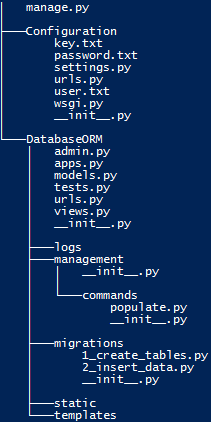
\includegraphics[scale = 0.75]{images/1.png}
	\caption{Структура проекта}
	\label{image:1}
\end{figure}

В проекте присутствует: главный файл проекта \emph{manage.py}; конфигурационный модуль \emph{Configuration}, содержащий конфигурационный файл \emph{settings.py}; основной модуль, содержащий описание моделей (\emph{models.py}), собственные команды (\emph{management/commands/*}), миграции (\emph{migrations/*}) и др.

Изменения в конфигурационном файле:

\lstinputlisting{listings/settings.py}

Логин, пароль и секретный ключ хранятся в специальных файлах, которые не добавляются в систему контроля версий. Также в базу данных по умолчанию добавляется несколько таблиц, связанных с аутентификацией.

\subsection{Миграция базы данных}

С помощью механизма миграций воссоздадим следующую схему базы данных:

\begin{figure}[h!]
	\centering
	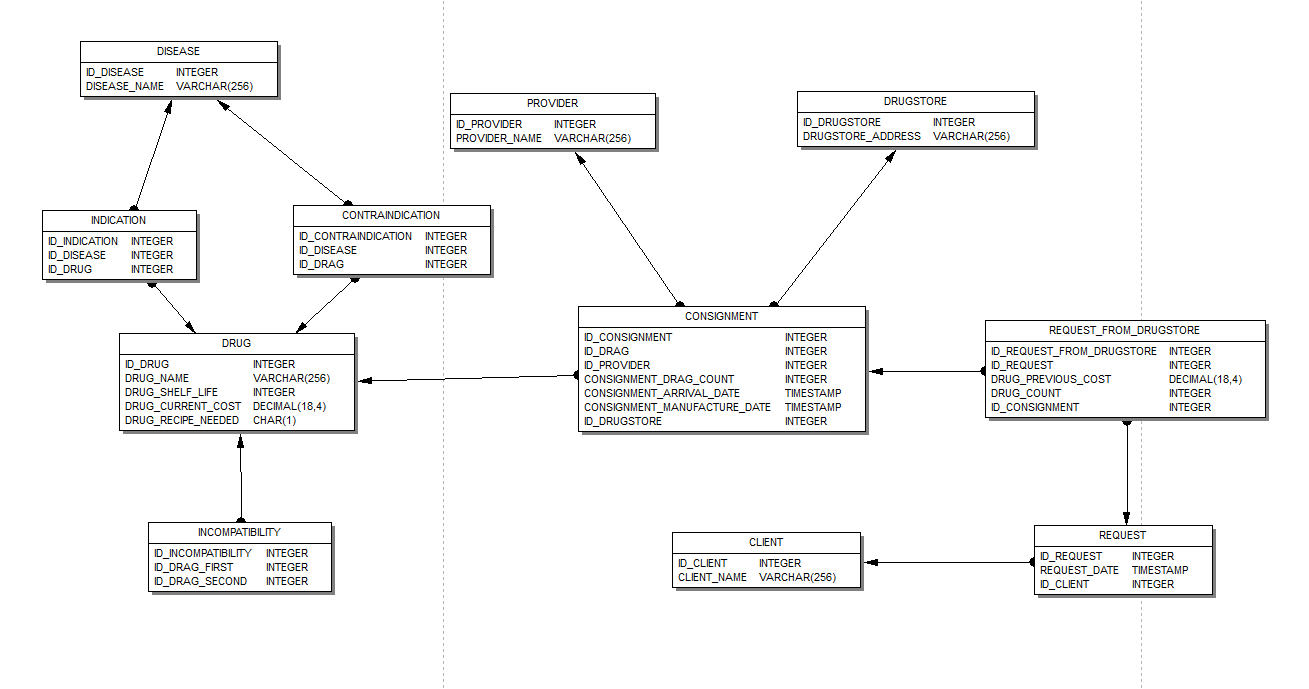
\includegraphics[scale = 0.50]{images/2.png}
	\caption{Схема базы данных}
	\label{image:2}
\end{figure}

Опишем модели в файле \emph{models.py}:

\lstinputlisting{listings/models.py}

После этого была создана миграция командой \emph{makemigrations}, переименуем миграцию \emph{0001\_initial.py} в \emph{1\_create\_tables.py} для большей читабельности.

Для запуска миграции воспользуемся следующим кодом:

\begin{figure}[h!]
	\centering
	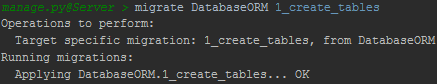
\includegraphics[scale = 0.95]{images/3.png}
	\caption{Запуск миграции}
	\label{image:3}
\end{figure}

\clearpage

Проверим, добавились ли таблицы:

\begin{figure}[h!]
	\centering
	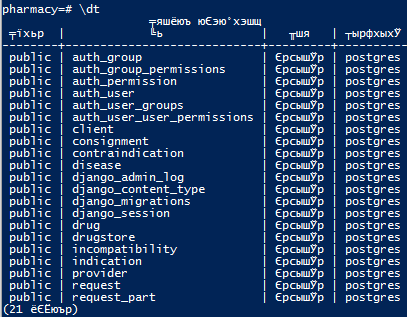
\includegraphics[scale = 0.85]{images/4.png}
	\caption{Созданные таблицы}
	\label{image:4}
\end{figure}

Откатим миграцию:

\begin{figure}[h!]
	\centering
	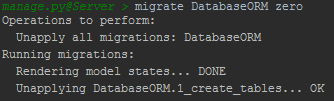
\includegraphics[scale = 0.95]{images/5.png}
	\caption{Откат миграции}
	\label{image:5}
\end{figure}

Проверим, удалились ли таблицы:

\begin{figure}[h!]
	\centering
	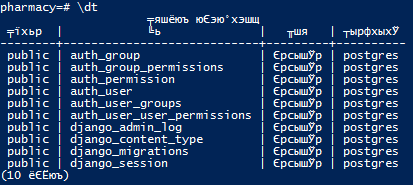
\includegraphics[scale = 0.85]{images/6.png}
	\caption{Оставшиеся таблицы}
	\label{image:6}
\end{figure}

\subsection{Добавление данных}

Попробуем добавить данные двумя способами: с помощью миграций и с помощью команд. 

Была создана миграция \emph{2\_create\_data.py}, в которой в таблицы добавляются данные:

\begin{figure}[h!]
	\centering
	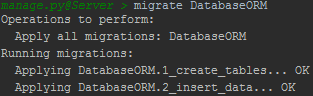
\includegraphics[scale = 0.95]{images/7.png}
	\caption{Запуск всех миграций}
	\label{image:7}
\end{figure}

Были созданы таблицы с данными:

\begin{figure}[h!]
	\centering
	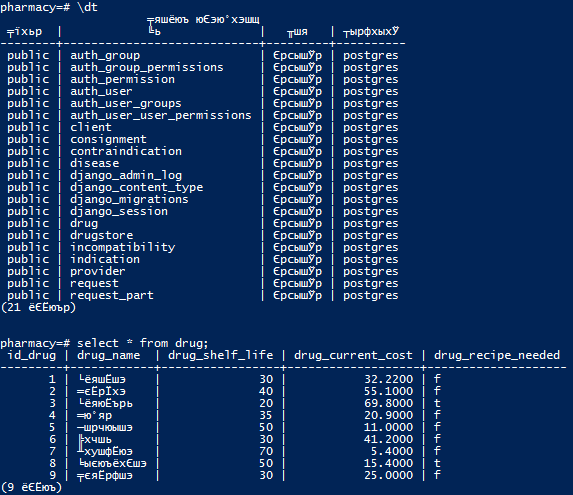
\includegraphics[scale = 0.80]{images/8.png}
	\caption{Созданные таблицы с данными}
	\label{image:8}
\end{figure}

Однако, в миграции обычно добавляют только важнейшие данные, которые не будут изменяться. Для добавления обычных данных в таблицы рекомендуется использовать \emph{manage commands}:

\lstinputlisting{listings/populate.py}

Теперь можно миграцией создать таблицы, после чего командой  добавить данные:

\begin{figure}[h!]
	\centering
	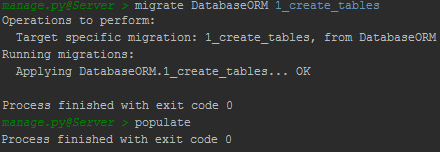
\includegraphics[scale = 0.80]{images/9.png}
	\caption{Создание таблиц и добавление данных}
	\label{image:9}
\end{figure}

\section{Вывод}

В результате данной работы было проведено знакомство с миграциями моделей используя Django, а также с manage-командами для наполнения базы данных. К достоинствам миграции Django можно отнести:

\begin{itemize}
	\item Ускорение процесса изменения схемы базы данных.
	\item Возможность отслеживания схемы базы данных.
	\item Поддержка многими бэкендами (PostgreSQL, MySQL, SQLite).
	\item Возможность отката.
\end{itemize}

Также был проведен опыт использования manage-команд. Использование данного инструмента позволяет расширить проект, написанием каких-либо собственных команд. Так например, можно написать генератор для заполнения полей таблиц в базе данных.






\end{document}